% !TEX root = ../main.tex
\chapter{Twitter}
\label{ch:twitter}

\section{Introduction to Twitter}
\label{sec:twitter}

Twitter is a form of so-called microblogging, which is defined as a form of blogging with small-sized pieces of content,
usually text up to a character-count of 200, which in the case of Twitter are called Tweets or statuses.
This enables light-weight, mobile and easy sharing of opinions, status and activities~\cite{Finin2007},
which lead to rapid adoption and user growth~\cite{mcgiboney2009twitter}.
\par
As shown in~\ref{tab:comparison}, the relationships of following users and being followed by users on Twitter is unreciprocated,
which means it requires no active accepting of followers.\\
This leads to only 22.1\% of users being followed by someone, also follow that user back~\ref{Kwak2010}.
Although Twitter offers the option to protect ones account, which means followers need to be accepted,
and users can be blocked, thereby denying them seeing ones content, these options are only used in rare cases,
making the form of relationships they represent the exception~\ref{Kwak2010}.\\
The relationship between different kinds of entities present on Twitter can be seen in~\ref{fig:twitter}
\par

% include diagram
\begin{figure}
    \centering
    \caption{Simplified diagram of Twitter entity relations.}
    \label{fig:twitter}
    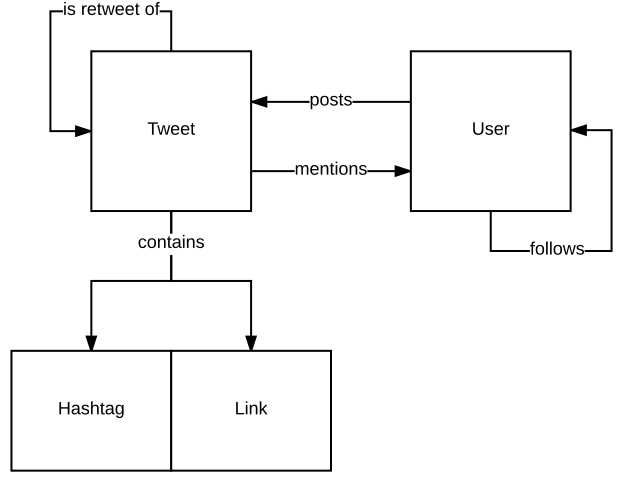
\includegraphics[width=10cm]{../figures/twitter_er.pdf}
\end{figure}

\par
% TODO statuses/tweets persistence
This thesis will focus on analyzing statuses in real time.
Statuses on Twitter can not only contain text, but also rich media like images, gifs, or videos, as well as surveys.
The text itself can also contain links, mention other users by containing \texttt{@<user_name>},
and contain any number of the infamous hashtag (\texttt{#hastag}), used to label a status, all while being limited to 140 characters.
A status can also be a so-called retweet of another status, adding to its content and exposing the other status to the retweeting users' followers.
Research shows that statuses are mostly retweeted shortly after they are published, and often lead to chains of retweets,
which not only spreads information fast, but also diffuses it~\ref{Kwak2010}.\\
As mentioned in~\ref{ch:goals}, one of the goals of this thesis is to be able to observe and detect such a spreading in real time
and analyze its influence on the overall userbase.
\par
For the purpose of this thesis we will only focus on the text of a status and do not assign any special meaning to links,
mentions, hashtags or whether a status is a retweet.\\


\section{The Twitter API}
\label{sec:theApi}

Twitter is offering an API (\textbf{A}pplication \textbf{P}rogramming \textbf{I}nterface),
through which developers and researchers can access machine-readable data,
including the entities shown in~\ref{fig:twitter}, from the platform.
This API transmits data encoded in JSON, and follows the REST-paradigm.

\subsection{JSON}
\label{subsec:json}

JSON (\textbf{J}ava\textbf{S}cript \textbf{O}bject \textbf{N}otation) is data format originally conceptualized by ECMA international
for the programming language Javascript to be light-weight, human-readable yet easy for machines to generate and parse.
Due to this, and the fact that it uses conventions familiar to developers of C-like languages,
it has since become a widespread data-interchange format with libraries for parsing and generation in many languages~\cite{jsonDocs}.
A small example for an object in this format can be seen in~\ref{code:json}.


%{
%    "apple": {
%        "calories": 123,
%        "contains_allergens": false
%        "types": ["Braeburh", "Cortland"]
%        "grows_on": "tree"
%    },
%    "hazelnut": {
%        "calories": 12,
%        "contains_allergens": true
%        "grows_on": "bush"
%    },
%}

\begin{figure}
    \caption{A shortened JSON representation of a fictional Twitter status}
    \label{code:json}
    \begin{minted}{json}
        % @formatter:off
    {
        "created_at" : "Fri Jan 20 20:04:05 +0000 2017",
        "id" : "123",
        "text" : "@other_user Hello!",
        "entities" : {
                "hashtags" : [],
                "symbols" : [],
                "user_mentions" : [{
                    "screen_name" : "other_user",
                    "name" : "Other User"}],
                "urls" : [] },
        "user" : {
            "name" : "User",
            "screen_name" : "user"
        }
    }
        % @formatter:on
    \end{minted}
\end{figure}

\subsection{REST}
\label{subsec:rest}

The Twitter API follows the REST (\textbf{RE}presentational \textbf{S}tate \textbf{T}ransfer) paradigm.
The REST-paradigm defines a set of architectural rules to ensure interoperability of distributed systems,
like clients and servers on the internet.
To achieve that, among other things,
it defines a set methods that specify different kinds of operations that can be performed on data~\cite{Jakl2008}.
The most prevalent methods mentioned in the RFC are listed below~\cite{RFC2616}.

\begin{enumerate}
    \item
    \texttt{GET} - retrieves data identified by the URI (idempotent)
    \item
    \texttt{POST} - request to create a new entity, with the type specified by the URI
    \item
    \texttt{PUT} - request to create an entity identified by the URL, or update it if it exists (idempotent)
    \item
    \texttt{DELETE} - request to delete an entity identified by the URL (idempotent)
\end{enumerate}

There are more methods specified by the RFC~\cite{RFC2616} that will not be used in this thesis.
\par
The resources (also called API endpoints) offered by the Twitter REST-API are rate-limit,
which means any one application or Twitter-user using the API can make a limit number of requests to the API.
Every request send to the API needs to be authenticated,
either as a Twitter user or as an application that can be registered in Twitter's developer console.
Furthermore, there are some resources which can only be accessed when a specific Twitter user authenticates
against the API, because they are user-specific, like publishing a status.
Some examples can be seen in ~\ref{tab:twitter_endpoints}.
% TODO this would be a good place to elaborate some more
% TODO the rate limiting part, for example, is kind of lost int here

\begin{table}
    \caption{A selection of resources offered by the Twitter REST API~\cite{twitterDocs}}
    \label{tab:twitter_endpoints}
    \resizebox{\textwidth}{!}{%
    \begin{tabular}{lllll} %
        \toprule
        & & \multicolumn{2}{c}{Authentication} & \\
        \cmidrule{3-4}
        Method
        & URI
        & User
        & Application
        & Description
        \\
        \midrule
        \texttt{GET}
        & \texttt{search/tweets}
        & \cmark
        & \cmark
        & Returns statuses matching a query
        \\
        \midrule
        \texttt{GET}
        & \texttt{direct_messages}
        & \cmark
        & \xmark
        & Returns direct messages of the authenticated user
        \\
        \midrule
        \texttt{POST}
        & \texttt{statuses/update}
        & \cmark
        & \xmark
        & Posts a status for the authenticated user
        \\
        \bottomrule
    \end{tabular}}
\end{table}

\subsection{Data at Rest - Data in Motion}
\label{subsec:dataAtRest-DataInMotion}


\subsection{Streaming}
\label{subsec:streaming}

But we want to do real time - that doesn't work properly with the REST API
- thankfully you can also stream twitter

(Dis-)Advantages of Streaming- and REST-API for this and other usecases (i.e. that it is realtime)

Explaining the different kinds of available streams plus parameters
Referencing ~\ref{subsec:kafka}: Compared to the general use case presented in~\ref{fig:kafka},
there is only one topic per producer, with the topic being the stream a user started and the produer being twitter.
(Show adjusted figure with one producer feeding into)

\section{The Sanders Dataset}
\label{sec:theSandersDataset}

Evaluation using the comparison in \cite{Saif2013} showed the sanders-dataset \cite{sanders} to be most-suited to train twitter sentiment analysis models.
Explaining the dataset.
The Sanders dataset is used for all models.
Reasons: to ensure consistency, and because it is hand-labeled (important for sentiment analysis, and also labeling by other means, e.g. emoticons, is flawed)

\begin{itemize}
    \item
    Hydration of the dataset and why it was required (because of Twitter TOS)
    \item
    The original crawling script for the sanders data set was not working due to breaking changes in the api, a fixed version would take 9 hours, a short yet efficient script was created to get the tweets
    \item
    Filtering of the dataset removing e.g. non-english tweets
\end{itemize}

Perform some preliminary data exploration: Wordcloud, some actual tweets showing sentiment regarding specific topics for a keyword, most used/least used words, etc.
Generally giving the reader a feeling for the data we are working with here.
Giving a convincing argument why it makes sense to use it.

\section{The Streaming Sample Dataset}
\label{sec:streamingSampleDataset}

Another dataset was collected by listening to the sample stream with the same filter settings as used on the sanders dataset.
In this case this meant only keeping english tweets.
This is done until N tweets are collected.

Do the same sort of exploration as with the Sanders Dataset, but additionally showing a graph of number of incoming tweets over time for a keyword or something like that

\section{Preprocessing and Tokenization}
\label{sec:preprocessingAndTokenization}

There are now 2 datasets of "raw", but filtered tweets.
Pointing out flaws in the dataset encoutered during exploration.

\begin{itemize}
    \item
    For consistency, the same preprocessing and tokenization functions are used for training, testing and streaming for all models and algorithms
    \item
    Explaining how it was difficult to clean up the tweets (with examples)
    \item
    Show actual preprocessing code, since its a vital piece and not that long
    \item
    Graphics of preprocessed data for both datasets in the same visualizations as during exploration, with comparison, proving the effectiveness of the preprocessing
    \item
    2 Gensim-Dictionaries were made, one from the actual Stream Dataset, one from the Sanders dataset, for sentiment analysis and lda topic modeling, in the same format to test them against each other later.
    Is it okay to only briefly explain what a Gensim-Dictionary is here?
    Because Gensim is primarily used for LDA, and is exaplained in detail there.
    \item
    Explaining the saving of the preprocessed tweets and dictionaries (persistence layer)
\end{itemize}

3 pages planned for this chapter.
\pagebreak[3]